\documentclass[a4paper,12pt]{article}
\usepackage{général}
%
\usepackage[french]{babel}
% \usepackage[T1]{fontenc}
% \usepackage[utf8]{inputenc}
%
% \usepackage[margin=3cm,tmargin=5cm,bmargin=3.5cm]{geometry}
%
% \usepackage{hyperref}
%
% \usepackage{graphicx}
%
\usepackage{color}

\title{
    \begin{figure}[!t]
    \begin{minipage}{.25\textwidth}
    
\includegraphics[width=\textwidth]{img/logo_lmu.png}
    \end{minipage}
    \hspace{.5\textwidth}
    \begin{minipage}{.25\textwidth}
    
\includegraphics[width=\textwidth]{img/logo_ic2.png}
    \end{minipage}
    \end{figure}
    \begin{center}
	\textbf{\textcolor{blue}{Le Mans Université}} \\
	Licence Informatique \textit{2ème année} \\
	Module 174UP02 Rapport de Projet \\
	\textbf{Titre du projet}
    \end{center}
}
\author{
	\begin{tabular}{rl}
	    Matthieu & \textsc{Boulanger} \\
	    Ania & \textsc{Garoui} \\
	    Yohan & \textsc{Harison} \\
	    Jacques-Gérard & \textsc{Mpondo Toutou}
	\end{tabular}
}
\date{\today}

\begin{document}

\maketitle
\newpage

\tableofcontents
\newpage

\abstract{Ceci est le texte de mon résumé...}

\section{Introduction}

\textit{Cette introduction présentera le sujet qui sera traité et le travail avec une présentation du plan adopté} \\
Ce document présente un projet de jeu XXX réalisé dans le cadre de la formation de L2 informatique de l’université du Mans pendant la d-période de janvier à avril 2024.
Ce projet a été développé en langage C avec la librairie SDL.
Ce jeu fait ceci cela ... \\
Nous présenterons dans une première partie notre jeu , des scénarios d’utilisation et les principales fonctionnalités puis dans une deuxième partie la gestion du projet ensuite dans une troisième partie les éléments principaux de conception (algorithmes,structures de données, .....) ensuite nous présenterons l’architecture de notre application (structuration du code en fichiers) enfin nous montrerons les principaux résultats.
Enfin nous présenterons en conclusion les points forts et les limites de notre travail, les écarts entre la planification prévisionnelle et le déroulement réel de notre projet et les leçons tirés de cette expérience. En annexe nous présenterons un exemple de débogage et des tests ( jeux d’essai et cas de test d’un exemple au moins - le fichier .c étant dans le git dans un répertoire dédié "test") ....

\section{Partie 1}

Dans cette première partie nous allons présenter .... . La figure \ref{mon_image} illustre .....
\begin{figure}[h]
    \begin{center}
	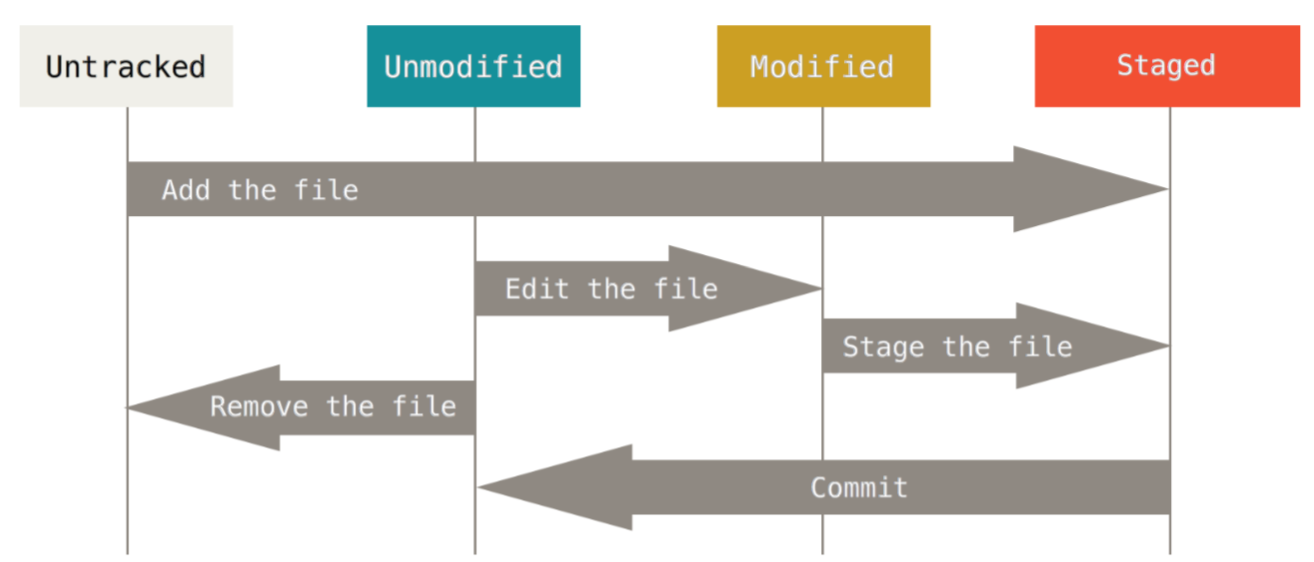
\includegraphics[width=.85\textwidth]{img/mon_image.png}
	\caption{mon image}
	\label{mon_image}
    \end{center}
\end{figure}

L’instruction \texttt{\textbackslash begin figure[!h]} force l’image à se positionner comme on le désire. Le positionnement de l’image dépend également de ses dimensions, si elle est située en bas de page, et qu’elle est trop grande, elle va se positionner sur la page suivante et le texte qui suit se retrouvera donc avant l’image.
Il faudra réduire la taille.
Ceci peut se faire avec l’option scale de \texttt{includegraphics}.

\subsection{Sous titre 1}
\subsection{Sous titre 2}

\section{Partie2- Les tableaux en Latex}

Les algorithmes de \LaTeX pour mettre en forme les tableaux ont quelques
imperfections. L’une d’entre elles est qu’il ne mettra pas automatiquement
le texte sur plusieurs lignes dans les cellules, même si celui-ci déborde de la
largeur de la page. Pour les colonnes qui contiendront une certaine quantité
de texte, il est recommandé d’employer l’attribut p et d’indiquer la largeur
désirée de la colonne (bien que cela puisse obliger à effectuer quelques ajustements avant d’obtenir le résultat escompté) (figure \ref{tableau_simple} et figure \ref{autre_tableau} ou figure \ref{autre_tableau_bis}) \cite{wikibooks} \cite{wikibooks}. ...

\begin{table}[h]
    \centering
    \begin{tabular}{|l|c|r|}
	\hline
	Un titre de colonne & Un autre titre & Un dernier \\
	\hline
	à gauche & centré & à droite \\
	\hline
	d & e & f \\
	\hline
	Si j’écris plus de texte je dépasse la taille de la page & texte & texte \\
	\hline
    \end{tabular}
    \caption{Un tableau simple}
    \label{tableau_simple}
\end{table}

\begin{table}[h]
    \centering
    \begin{tabular}{|c|p{3cm}|}
	\hline
	1 - 1 & Du texte \\
	\hline
	2 - 1 & On met un grand texte qui sera sur plusieurs lignes \\
	\hline
    \end{tabular}
    \caption{Un autre tableau}
    \label{autre_tableau}
\end{table}

% \begin{table}[h]
%     \centering
%     \begin{tabular}{|c|m{3cm}|}
% 	\hline
% 	colonne 1 & colonne "M" \\
% 	\hline
% 	court texte & Texte plus long qui sera centré dans la ligne et aligné à gauche dans la colonne \\
% 	\hline
%     \end{tabular}
%     \caption{Un autre tableau bis}
%     \label{autre_tableau_bis}
% \end{table}

\section{....}

\section{Conclusion}

\section{Glossaire ou lexique}

si nécessaire

\section{Bibliographie}

Veillez à citer les sources bibliographiques d’où vous extrayez des informations dans le coeur de votre article et les référencer explicitement dans cette partie.
Consultez les documents mis à disposition (Rédaction d’une biblio) pour la
mise en forme de cette bibliographie (cf Normes APA) \cite{apa_scribbr} \cite{apa_umontreal}.
Vous pouvez utiliser un fichier .bib pour insérer votre bibliographie, et
citer vos références de la manière suivante : \cite{Gre93}

\section{Annexe}

\begin{thebibliography}{REF}
    \bibitem{apa_scribbr}\url{https://www.scribbr.fr/category/normes-apa/}
    \bibitem{apa_umontreal}\url{https://bib.umontreal.ca/citer/styles-bibliographiques/apa?tab=3281} 
    \bibitem{wikibooks}\url{https://fr.wikibooks.org/wiki/LaTeX/Tableaux}
    \bibitem{zestedesavoir}\url{https://zestedesavoir.com/tutoriels/826/introduction-a-latex/1322_completer-vos-documents/images-tableaux-et-texte-preformate/#2-tableaux}
\end{thebibliography}
\end{document}
